\documentclass[journal]{vgtc}                % final (journal style)
%\documentclass[review,journal]{vgtc}         % review (journal style)
%\documentclass[widereview]{vgtc}             % wide-spaced review
%\documentclass[preprint,journal]{vgtc}       % preprint (journal style)

%% Uncomment one of the lines above depending on where your paper is
%% in the conference process. ``review'' and ``widereview'' are for review
%% submission, ``preprint'' is for pre-publication, and the final version
%% doesn't use a specific qualifier.

%% Please use one of the ``review'' options in combination with the
%% assigned online id (see below) ONLY if your paper uses a double blind
%% review process. Some conferences, like IEEE Vis and InfoVis, have NOT
%% in the past.

%% Please note that the use of figures other than the optional teaser is not permitted on the first page
%% of the journal version.  Figures should begin on the second page and be
%% in CMYK or Grey scale format, otherwise, colour shifting may occur
%% during the printing process.  Papers submitted with figures other than the optional teaser on the
%% first page will be refused.

%% These few lines make a distinction between latex and pdflatex calls and they
%% bring in essential packages for graphics and font handling.
%% Note that due to the \DeclareGraphicsExtensions{} call it is no longer necessary
%% to provide the the path and extension of a graphics file:
%% \includegraphics{diamondrule} is completely sufficient.
%%
\ifpdf%                                % if we use pdflatex
  \pdfoutput=1\relax                   % create PDFs from pdfLaTeX
  \pdfcompresslevel=9                  % PDF Compression
  \pdfoptionpdfminorversion=7          % create PDF 1.7
  \ExecuteOptions{pdftex}
  \usepackage{graphicx}                % allow us to embed graphics files
  \DeclareGraphicsExtensions{.pdf,.png,.jpg,.jpeg} % for pdflatex we expect .pdf, .png, or .jpg files
\else%                                 % else we use pure latex
  \ExecuteOptions{dvips}
  \usepackage{graphicx}                % allow us to embed graphics files
  \DeclareGraphicsExtensions{.eps}     % for pure latex we expect eps files
\fi%

%% it is recomended to use ``\autoref{sec:bla}'' instead of ``Fig.~\ref{sec:bla}''
\graphicspath{{figures/}{pictures/}{images/}{./}} % where to search for the images

\usepackage{microtype}                 % use micro-typography (slightly more compact, better to read)
\PassOptionsToPackage{warn}{textcomp}  % to address font issues with \textrightarrow
\usepackage{textcomp}                  % use better special symbols
\usepackage{mathptmx}                  % use matching math font
\usepackage{times}                     % we use Times as the main font
\renewcommand*\ttdefault{txtt}         % a nicer typewriter font
\usepackage{cite}

\usepackage[table]{xcolor} 
\usepackage{booktabs}
\usepackage{tikz}
\def\checkmark{\tikz\fill[scale=0.4](0,.35) -- (.25,0) -- (1,.7) -- (.25,.15) -- cycle;} 
\usepackage{algorithm}
\usepackage[noend]{algpseudocode}
\usepackage{color}

\usepackage{titlesec}
\usepackage{verbatim}
\usepackage{enumitem}
\setlist[enumerate]{itemsep=0mm}

\titlespacing\subsubsection{0pt}{4pt plus 4pt minus 2pt}{0pt plus 2pt minus 2pt} %11

\titlespacing\section{0pt}{8pt plus 4pt minus 2pt}{1pt plus 1pt minus 1pt}

\titlespacing\subsection{0pt}{4pt plus 4pt minus 2pt}{1pt plus 1pt minus 1pt}

%% We encourage the use of mathptmx for consistent usage of times font
%% throughout the proceedings. However, if you encounter conflicts
%% with other math-related packages, you may want to disable it.

%% In preprint mode you may define your own headline.
%\preprinttext{To appear in IEEE Transactions on Visualization and Computer Graphics.}


%%% Put your definitions there:
%\startlocaldefs
\newcommand{\theName}{\textit{BioLinker}}
\newcommand{\theNames}{\textit{BioLinker}}
%\def \theTitle XXX
%\endlocaldefs


%% If you are submitting a paper to a conference for review with a double
%% blind reviewing process, please replace the value ``0'' below with your
%% OnlineID. Otherwise, you may safely leave it at ``0''.
\onlineid{128}

%% declare the category of your paper, only shown in review mode
\vgtccategory{Application}

%% Paper title.
\title{BioLinker: Bottom-up Exploration of Protein Interaction Networks}

\author{Tommy Dang\thanks{e-mail: tommy.dang@ttu.edu}\\ %
        \scriptsize Department of Computer Science \\ \scriptsize Texas Tech University %
\and Paul Murray\thanks{e-mail: pmurra5@uic.edu}\\ %
     \scriptsize Department of Computer Science \\ \scriptsize University of Illinois at Chicago %
\and Angus Forbes\thanks{e-mail: aforbes@uic.edu}\\ %
     \scriptsize Department of Computer Science \\ \scriptsize University of Illinois at Chicago %
} %
     
%% This is how authors are specified in the journal style

%% indicate IEEE Member or Student Member in form indicated below
%\author{}

%other entries to be set up for journal
%\shortauthortitle{Biv \MakeLowercase{\textit{et al.}}: Global Illumination for Fun and Profit}
%\shortauthortitle{Firstauthor \MakeLowercase{\textit{et al.}}: Paper Title}

%% Abstract section.
\abstract{Systems biologists and cancer researchers require interactive visualization tools that enable them to more easily navigate and discover patterns at different levels of the biological hierarchy of signaling pathways. Furthermore, biologists are often interested in understanding and exploring the causal biochemical links between processes. When exploring the literature of particular biological pathways or specific proteins within those pathways, biologists find it useful to know the contexts in which biochemical links are active and, importantly, to be aware of potential conflicts when different experiments introduce alternative interpretations of the function of a pathway or biochemical reaction. We introduce \theName{}, a interactive visualization system that helps users to perform bottom-up exploration of complex protein interaction networks. Five interconnected views provide the user with a range of ways to explore pathway data, including views that show potential conflicts within pathway databases and publications and that highlight contextual information about individual proteins. Additionally, we discuss system details to show how our system manages the large amount of protein interactions extracted from the literature of biological pathways. 

%The complete API functions are available at \url{http://ccrg-data.evl.uic.edu/index-cards/explorer}. 
%\parttitle{Conclusions} \theName{} is available as an online web application. The software, source code, and a demonstration video can be found via our GitHub project repository, located at \url{https://github.com/CreativeCodingLab/BioLinker}


} % end of abstract

\keywords{Protein interaction network, Dynamic network visualization, Potential conflict matrix.}

%% ACM Computing Classification System (CCS). 
%% See <http://www.acm.org/class/1998/> for details.
%% The ``\CCScat'' command takes four arguments.

\CCScatlist{ % not used in journal version
 \CCScat{K.6.1}{Management of Computing and Information Systems}%
{Project and People Management}{Life Cycle};
 \CCScat{K.7.m}{The Computing Profession}{Miscellaneous}{Ethics}
}

%% Uncomment below to disable the manuscript note
%\renewcommand{\manuscriptnotetxt}{}

%% Copyright space is enabled by default as required by guidelines.
%% It is disabled by the 'review' option or via the following command:
% \nocopyrightspace

%\vgtcinsertpkg

%%%%%%%%%%%%%%%%%%%%%%%%%%%%%%%%%%%%%%%%%%%%%%%%%%%%%%%%%%%%%%%%
%%%%%%%%%%%%%%%%%%%%%% START OF THE PAPER %%%%%%%%%%%%%%%%%%%%%%
%%%%%%%%%%%%%%%%%%%%%%%%%%%%%%%%%%%%%%%%%%%%%%%%%%%%%%%%%%%%%%%%%

\begin{document}

%% The ``\maketitle'' command must be the first command after the
%% ``\begin{document}'' command. It prepares and prints the title block.

%% the only exception to this rule is the \firstsection command

\firstsection{Introduction}

\maketitle

Molecular and systems biologists are tasked with the comprehension and analysis of incredibly complex networks of biochemical interactions, called pathways, that occur within every cell. It quickly becomes unwieldy to represent even a subset of all interactions between proteins, complexes, and biochemical reactions within a pathway, resulting in a visually cluttered ``hairball'' of tangled edge crossings. It is highly desirable to have interactive navigation tools to more effectively inspect the complex biological networks. In this paper, we propose \theName{}, a system that facilitates a bottom-up exploration of protein interaction networks. A user can initiate an exploration from a small subnetwork that encircles a particular protein of interest and then iteratively expand the network on demand by choosing individual elements. \theName{} provides multiple views that each display a different aspect of the currently selected subnetwork, such as the contexts of the protein interactions and the publication data related to the discovery of these interactions. These views are all linked to provide important supplementary information through brushing and linking.

We also describe the underlying infrastructure that allows \theName{} to load and filter the large amount of biological data at interactive rates. Our database currently contains over 3.5 million protein interactions extracted from more than 290,000 publications. The complete API functions are available at \url{http://ccrg-data.evl.uic.edu/index-cards/explorer}.

\section{Related Work}
%The analysis of pathway data is a critical component in the study of biological processes~\cite{saraiya2005visualizing}. For example, cancer biologists study mutations that perturb pathways involved in regulating cell growth, replication and mediated cell death~\cite{cairns2011regulation}. Research in drug development also involves analyzing how proteins targeted by a drug interaction modify the cellular behavior of a pathway in desired ways and avoid unintended downstream consequences~\cite{luo2003targeting}. Additionally, in order to program adult stem-cells so that they develop into functional tissue, researchers need to initiate pathways that precipitate cellular differentiation into specific cell types~\cite{reya2001stem}. 

Pathways may contain dozens or even hundreds of biomolecules. Reactions between these biomolecules include state transitions, such as activation, and frequently involve multiple inputs and outputs.  While some reactions can be usefully thought of as taking place one after another, in a linear series of steps, others are more accurately modeled as feedback loops~\cite{biovisDang2} where the outputs from one stage inhibit or activate the inputs to another stage. Furthermore, a system-level understanding of a complex pathway involves a more holistic understanding than depicting individual interactions may provide. Visualizing complexity while also presenting a high-level overview of such protein interaction networks is a significant challenge~\cite{saraiya2005visualizing}.

To tackle these challenges, numerous visualization techniques have been proposed. \textit{PathwayMatrix}~\cite{biovisDang1} represents binary relations between pairs of proteins and biomolecules. Various strategies are used to reorder proteins in the matrix; this enables the identification network structures which is difficult to extract using traditional node-link diagrams
with force-directed layouts, such as \textit{PCViz}~\cite{cerami2011pathway} or \textit{VisANT}~\cite{hu2009visant}. However, a drawback of matrix representations of networks is that it is difficult to trace a path between nodes. In contrast, \textit{RectionFlow}~\cite{biovisDang2} emphasizes both the structural and causal relationships among proteins, complexes, and biochemical reactions within a given pathway. Other hybrid forms, such as \textit{BioFabric}~\cite{longabaugh2012combing} and \textit{Compressed Adjacency Matrices}~\cite{dinkla2012compressed}, also attempt to reduce the number of edge crossings while enabling the traceability of network flows. 

Our scientific understanding of many signaling pathways is incomplete, both with respect to participating cellular components and their conditions (or \textit{context}, e.g., a pathway being active only during ``late phases of tumorigenesis''). Recent efforts in text mining focus on extracting causal mechanisms and contexts from research abstracts and scientific
papers~\cite{Valenzuela2015DBLP,Valenzuela:15,Valenzuela:16}. 
These efforts generate a large amount of data (millions of protein interactions together with context knowledge and expressions of uncertainty). Moreover, aligning this extracted evidence to existing databases of biochemical pathways, such as \textit{Pathway Commons}~\cite{PathwayCommons2011} and \textit{Wiki Pathways}~\cite{Kutmon2016WikiPathways}, is a daunting task. 

In this paper, we propose \theName{}, a system that facilitates a bottom-up exploration of protein interaction networks. A user can initiate an exploration from a small subnetwork that is connected to a particular protein of interest and then iteratively expand the network on demand by choosing individual elements. \theName{} provides multiple views that each displays a different aspect of the currently selected subnetwork, such as the contexts of the protein interactions and the publication data related to the discovery of these protein interactions. Each of these views--- \textit{overview}, \textit{main network view}, \textit{context view}, \textit{conflict matrix view}, and \textit{publication view}--- are all linked to provide important supplementary information through brushing and linking.
 
%We also describe the underlying infrastructure that allows \theName{} to load and filter the large amount of biological data at interactive rates. Our database currently contains over 3.5 million protein interactions extracted from close to 290 thousand publications. The complete API functions are available at \url{http://ccrg-data.evl.uic.edu/index-cards/explorer}
 
%The rest of this paper is organized as follows: We begin with an overview of visualization tasks. We then describe components in our system. We highlight the differences of \theName{} compared to related tools for protein network visualization. Finally, we conclude our paper with future plans. 
 
\section{Overview of Visualization Tasks}
We worked closely over a period of twelve months with three computational and molecular biologists to identify and prioritize visualization tasks in visualizing complex protein interaction networks. Our in-depth interviews with these experts led us to identify six important tasks that were not currently well-supported in existing visualization tools. The six visualization tasks, described in more detail later in the paper, include:
\begin{itemize}[noitemsep,nolistsep]
\item[\textbf{T1}]{Starting with specific protein, the visualization should allow users to iteratively expand the network on demand.}
\item[\textbf{T2}]{Overlaying cancer genomics data onto the network.}
\item[\textbf{T3}]{Finding the paths between two proteins based on user-specified number of hops.}
\item[\textbf{T4}]{Comparing protein interaction sub-networks by context.}
\item[\textbf{T5}]{Displaying publication data on request.}
\item[\textbf{T6}]{Enabling conflict detections in literature regarding protein interactions.}
\end{itemize}

The process of developing \theName{} was an iterative process that relied on feedback from the domain experts at various stages of the design and implementation. Many of the ideas that were included were first suggested by one of the domain experts, or emerged organically through conversations with them. The contributions of this paper are centered around building the software system that can handle the increasingly large amount of generated data and allow users to perform the above visualization tasks.

\section{Methods}
In this section we describe the primary components of the \theName{} visualization. \theName{} uses a client-server architecture to handle large amount of data from various databases. The server contains four components: 

%%%%%%%%%%%%%%%%%%%%%%% SERVER side
\begin{itemize}[noitemsep,nolistsep]
\item \textbf{Publication database}: We currently store over 290,000 PubMed articles on our server. % (Section~\ref{sec:PMC}).
\item \textbf{Index card database}: An \textit{index card} captures information, such as participants and interaction type, extracted from text in an article. Index cards are stored in structured data format to ensure that systems provide results in a single format that is computable but also human readable and editable. % (Section~\ref{sec:IndexCard}).
\item \textbf{Comparing index cards}: For every two given indexes, we identify if there are potential conflicts between them. A comparator script is deployed on our server for this purpose. % (Section~\ref{sec:Comparator}).
\item \textbf{Genomic alteration database}: \theName{} accesses the cBioPortal~\cite{cBioPortal2013} for Cancer Genomics through its web API. The portal was originally developed at Memorial Sloan-Kettering Cancer Center. %(Section~\ref{sec:cBioPortal}).
\end{itemize}

%%%%%%%%%%%%%%%%%%%%%%% CLIENT side
The client side contains five components (depicted in Fig.~\ref{fig:BioLinkerOverview}): 
\begin{itemize}[noitemsep,nolistsep]
\item \textbf{Overview/Protein Selector}: This panel allows users to select an initial protein.
\item \textbf{Main view}: Within this view, users can iteratively expand the network by clicking on individual protein names. % (Section~\ref{sec:MainView}).
\item \textbf{Context view}: This view shows statistics about the contexts of proteins (including species, cell type, organism) for the selected index cards in the main view.  %(Section~\ref{sec:ContextView}). 
\item \textbf{Publication view}: This view shows the discoveries related to how particular proteins interact with each other (as encapsulated by the index cards) and how our understanding of these interactions has changed over time.  %(Section~\ref{sec:PublicationView}).  
\item \textbf{Conflict matrix}: The index card comparisons are presented in form of an adjacency matrix. % (Section~\ref{sec:ConflictMatrix}). 
\end{itemize}

\begin{figure}[h!]
  \centering
  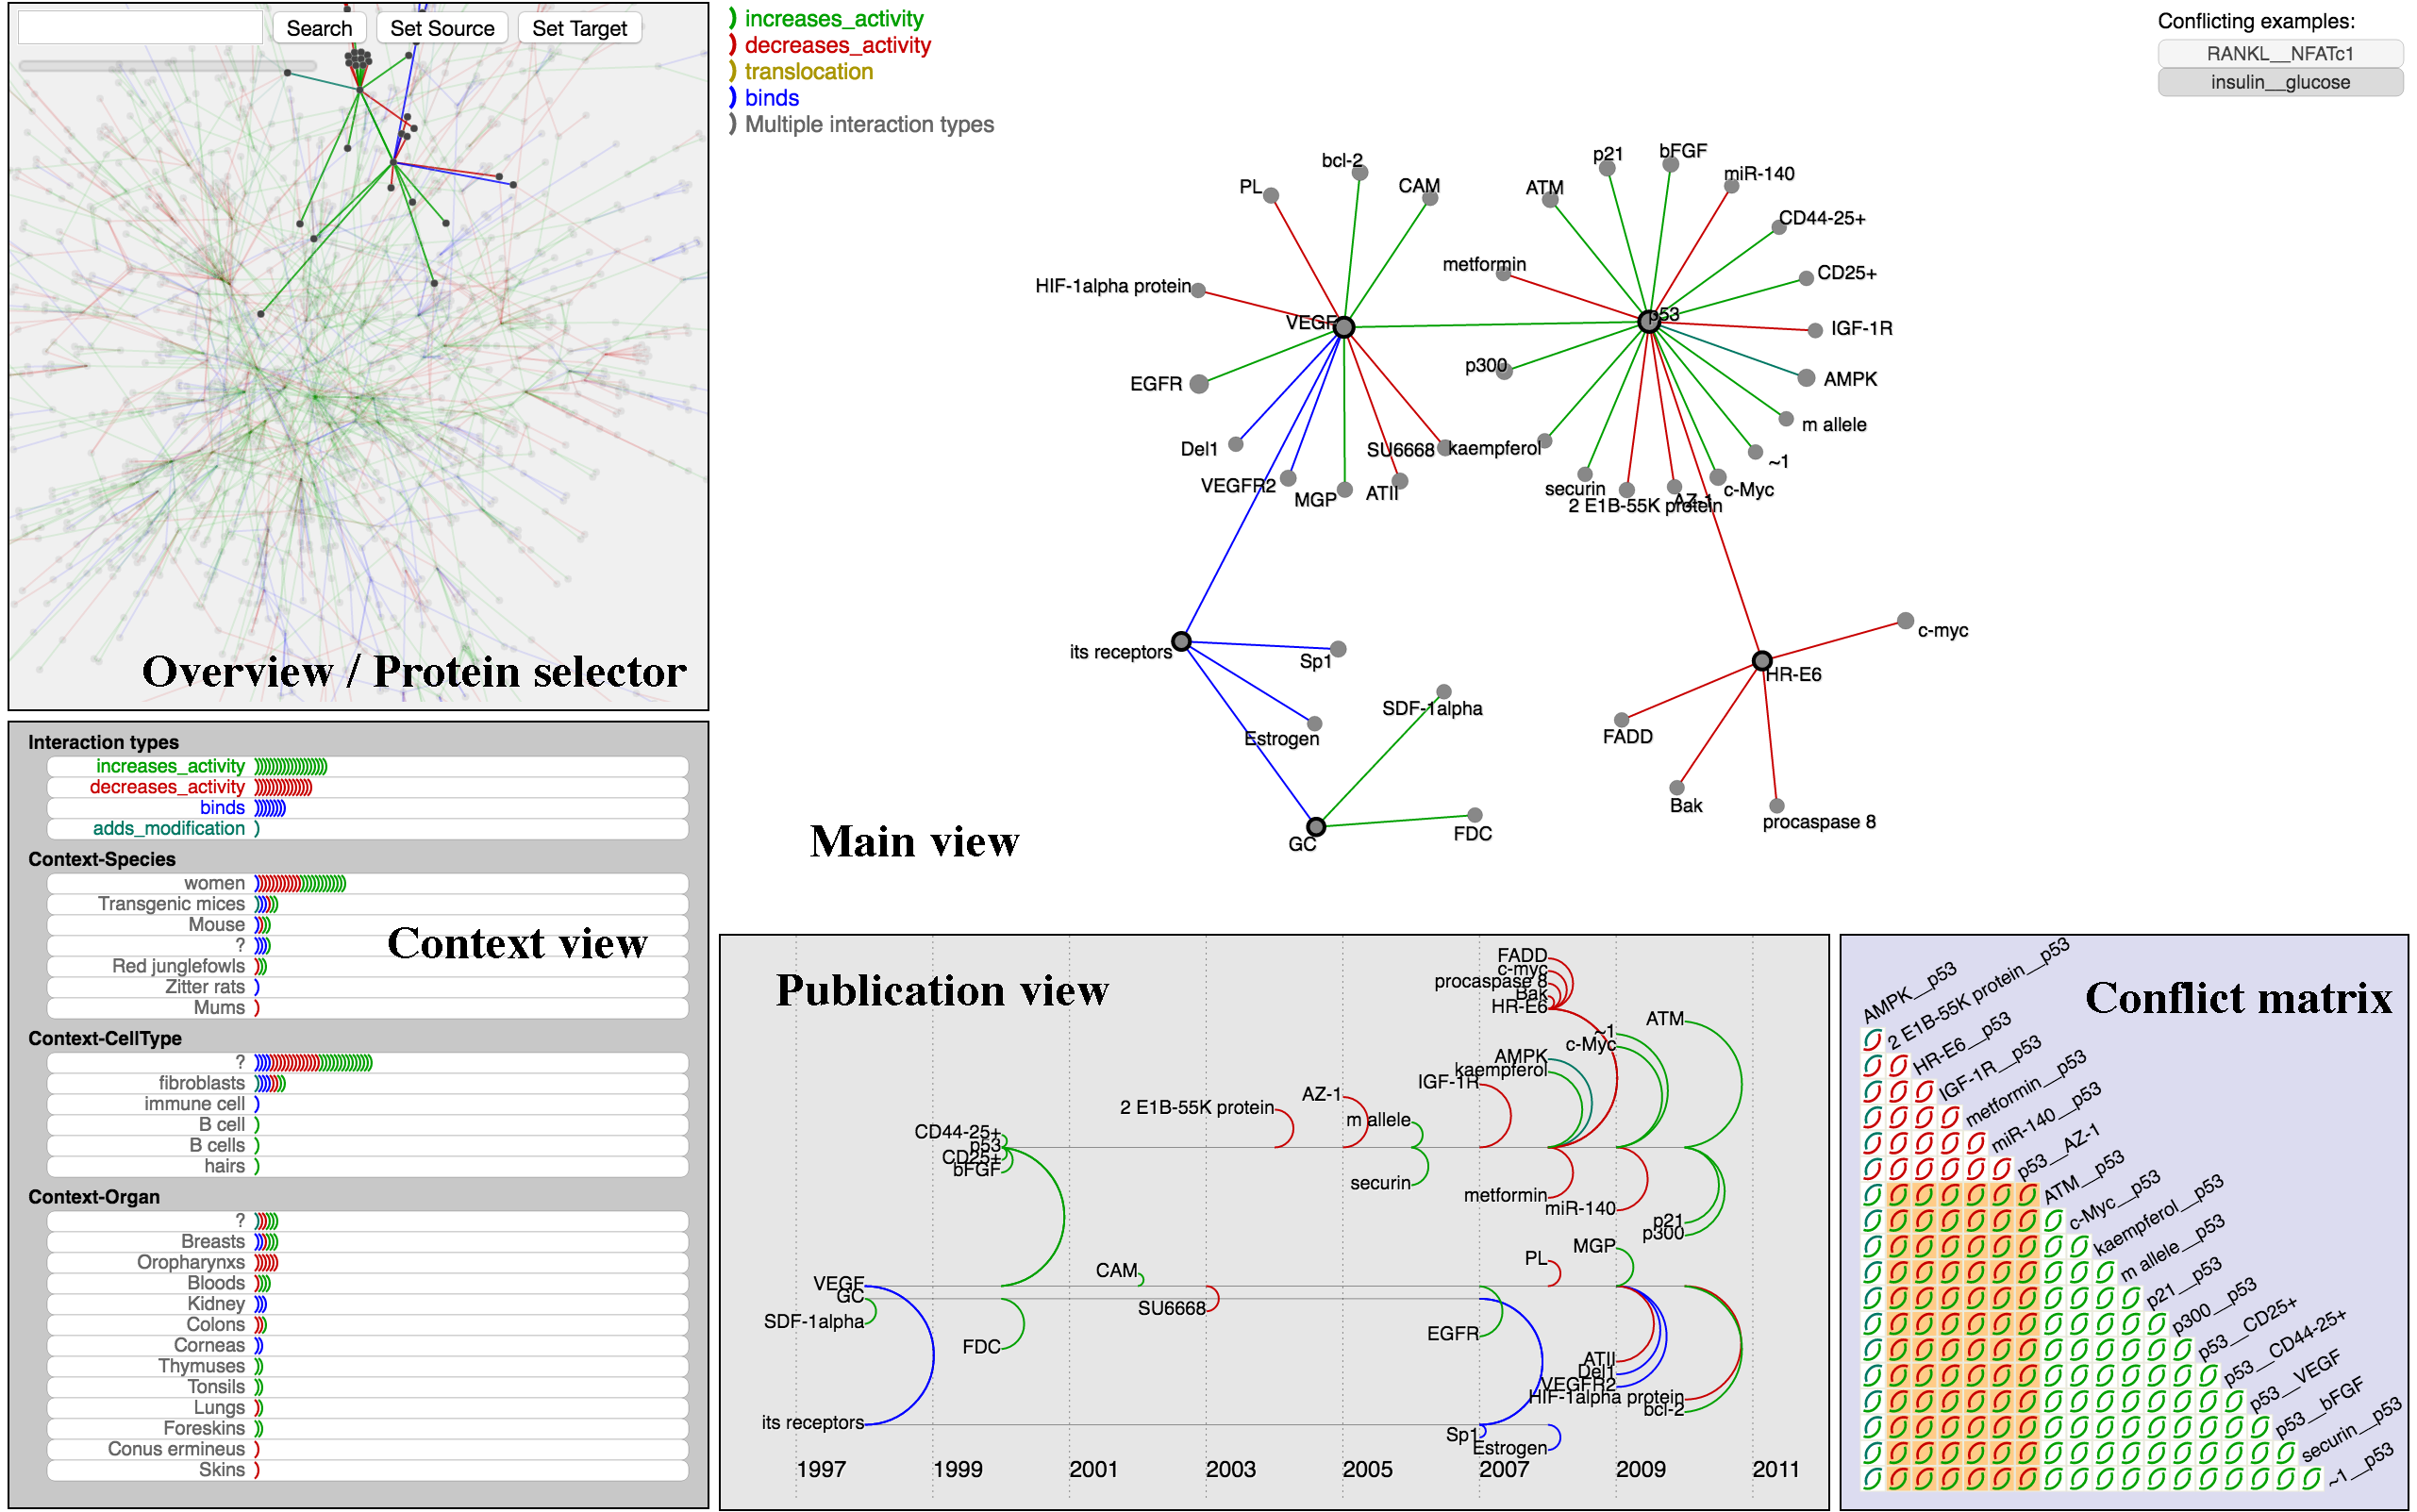
\includegraphics[width=250pt]{figures/Figure1.png}
  \caption{Client side of \theName{} visualization has multiple views.}
  \label{fig:BioLinkerOverview}
\end{figure}

These views are all interconnected through brushing and linking. For example, when a user selects a link (index card) between two proteins in the main view, the publication view shows the associated publication information (such as paper id, paper title, authors, journal name, and publication date) while the context view shows the species name, organ, and cell type for that protein interaction. 

\subsection{Publication database}
\label{sec:PMC}
PubMed Central (PMC) is a free full-text archive of biomedical and life sciences journal literature. We currently store over 290,000 PMC publications on our server. PMC uses XML tags to encode information about journal article submissions. These XML elements have specific style rules associated with them. There are many elements in a PMC publication, and we show the most important subset of these XML elements (as requested by our expert users), including the paper title, authors' names, authors' contact information and affiliations, publication year, journal name, and external link to the actual paper when it is available online. An example of PMC paper information stored on our server can be found at \url{http://ccrg-data.evl.uic.edu/index-cards/api/NXML/PMC1174968}.

\subsection{Index card database}
\label{sec:IndexCard}
The index card database is provided by the REACH Biomedical Information Extraction research group at University of Arizona. Their text extraction system automatically ``reads'' research papers and abstracts to construct causal models of biological pathway data and to facilitate the exploration and analysis of these models~\cite{Valenzuela:15,Valenzuela:16}. For each paper presented to the REACH reading system, a set of index cards is produced that capture the interactions reported in the paper along with the experimental evidence presented in the text as well as the relationships between the extracted interactions and the provided BioPAX model. 

An index card is a JSON object containing the following fields: participants, interaction type (binds, adds\_modification, removes\_modification, translocates), context (cell line, cell type, organism, tissue type), pmc\_id (the paper the result came from), evidence\_text (the text from the paper containing the information in the result.

Given that index cards are output in the JSON format, a MongoDB database is used to store index cards along with their associated publications (as PMC XML documents) and participants. The use of MongoDB also allows for a flexible document schema, which works well with the highly variable nature of index card documents. Since MongoDB does not support XML directly, PMC XML files are stored as binary objects. Index cards are stored in their raw form, and each index card is associated with the PMC XML document that it was extracted from. Each participant is also extracted from each index card and stored in a separate MongoDB collection, allowing for queries over participants.

A web API was created to serve index card, publication, and participant data. The API exposes a flexible query structure, allowing end users to query relations between index cards, participants, and PMC XML data in a variety of ways. An example of index cards on our server can be found at \url{http://ccrg-data.evl.uic.edu/index-cards/api/IndexCards/findOne}.


\subsection{Index cards comparator}
\label{sec:Comparator}
When there are multiple connections between two proteins/complexes, it may fall into one of the two following interesting circumstances: (1) If they have the same color (same interaction type), these are supporting evidences in different publications which confirm the interaction between two elements. (2) If they have the opposite colors (opposite interaction types, such as \textit{increase\_activity} versus \textit{decrease\_activity}). Domain experts are very interested in the latter case where there are conflicting evidences about the knowledge obtained from different publications (and usually in different years). 
We will show examples of the second circumstance below when we describe the conflict matrix and the publication view.  %Section~\ref{sec:ConflictMatrix} and \ref{sec:PublicationView}.

The above circumstance is just one specific example of conflicting evidences in literature about the interactions between proteins/complexes. We have deployed a more general comparator to detect potential conflicts on our server. Conflicts may happen between index cards of the same interaction type (for example, translocation but in the opposite direction) or different sets of participants (for example, one is a subset/member of another protein family participant). 

\subsection{Genomic alteration database}
\label{sec:cBioPortal}
The cBioPortal~\cite{cBioPortal2013} is hosted at and maintained by the Memorial Sloan Kettering Cancer Center. It provides access to data by the Cancer Genome Atlas as well as many carefully curated data sets. Currently, cBioPortal contains data from 147 cancer genomics studies (as of December 2016) and more than 17,000 tumor samples~\cite{ChiBE2_2014}. \theName{} accesses cBioPortal for Cancer Genomics through its web API. 

\subsection{Overview / Protein Selector}
\label{sec:ProteinSelector}
This panel provides an overview of thousand index cards sampled from millions of index cards in the database based on specified filtering conditions, such as protein interaction within the \textit{alphat} cell line. Users can start by entering a protein name into a search box (as depicted in the left panel of Fig.~\ref{fig:Figure2}). This will perform a request to load the selected protein and its immediate neighbors from our index card database. As users iteratively expand the subnetwork in the main view, the overview keeps track of the expanded sub-network over the overall context (as depicted in the right panel of Fig.~\ref{fig:Figure2}).

\begin{figure}[h!]
  \centering
  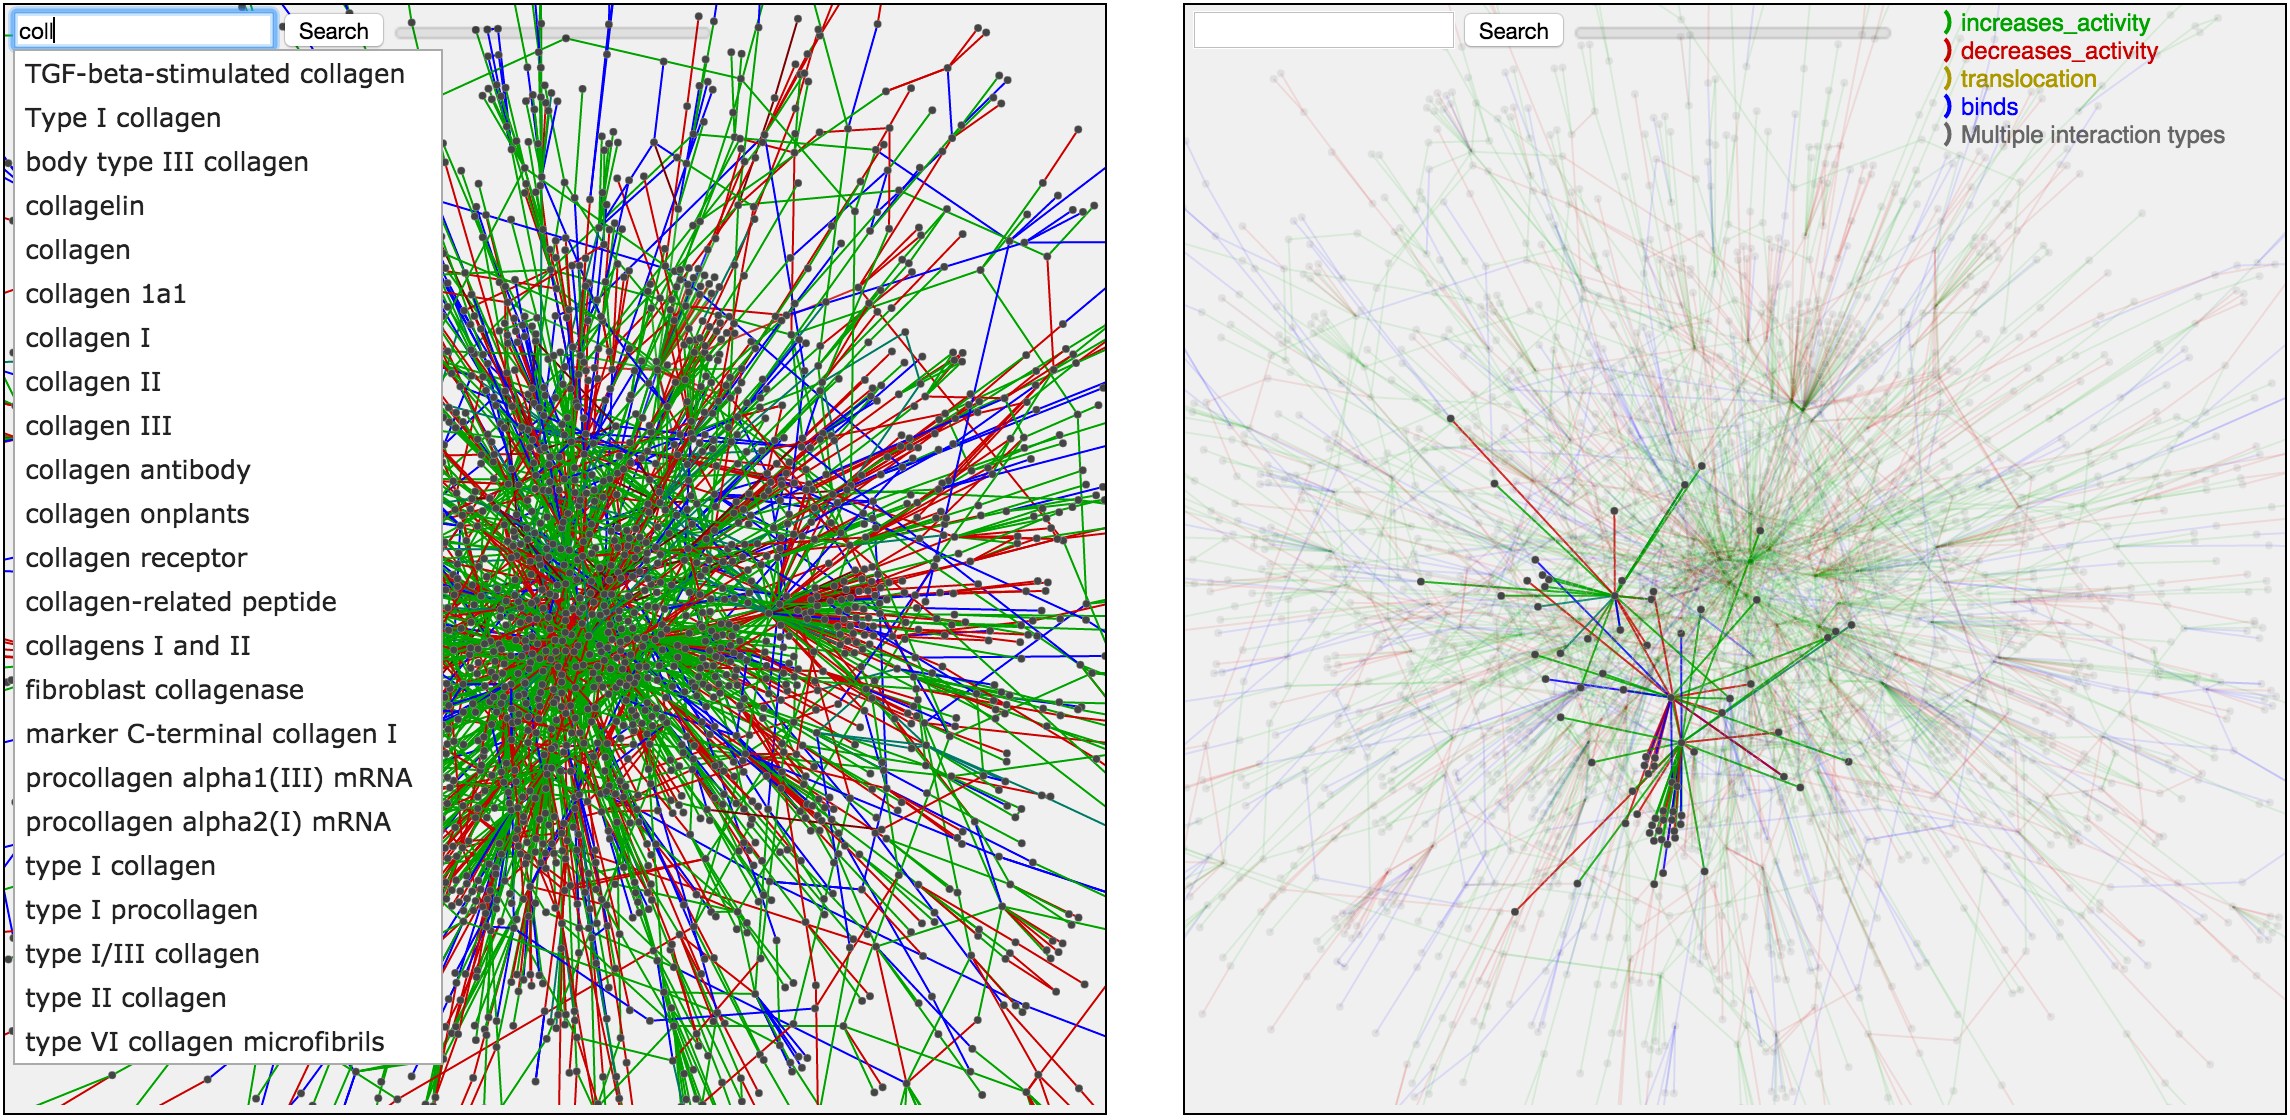
\includegraphics[width=250pt]{figures/Figure2.png}
  \caption{Protein selector (using the search box) in \theName{}.}
  \label{fig:Figure2}
\end{figure}

\subsection{Main View}
\label{sec:MainView}
A subnetwork encircling the selected protein is initially shown in the main view. Users can iteratively expand the network by simply clicking on protein names (visualization task \textbf{T1}). A query of relevant index cards (containing neighboring proteins) is sent to the index card database per user request. Node (protein) sizes are computed based on the number of direct neighbors. Edges (index cards) are color-encoded by interaction types, such as green for \textit{increase\_activity} and red for \textit{decrease\_activity}. When users mouse over a protein name, a pop-up window displays protein information together with statistics of its immediate neighbors (if expanded) as depicted in Fig.~\ref{fig:Figure3}.

\begin{figure}[h!]
  \centering
  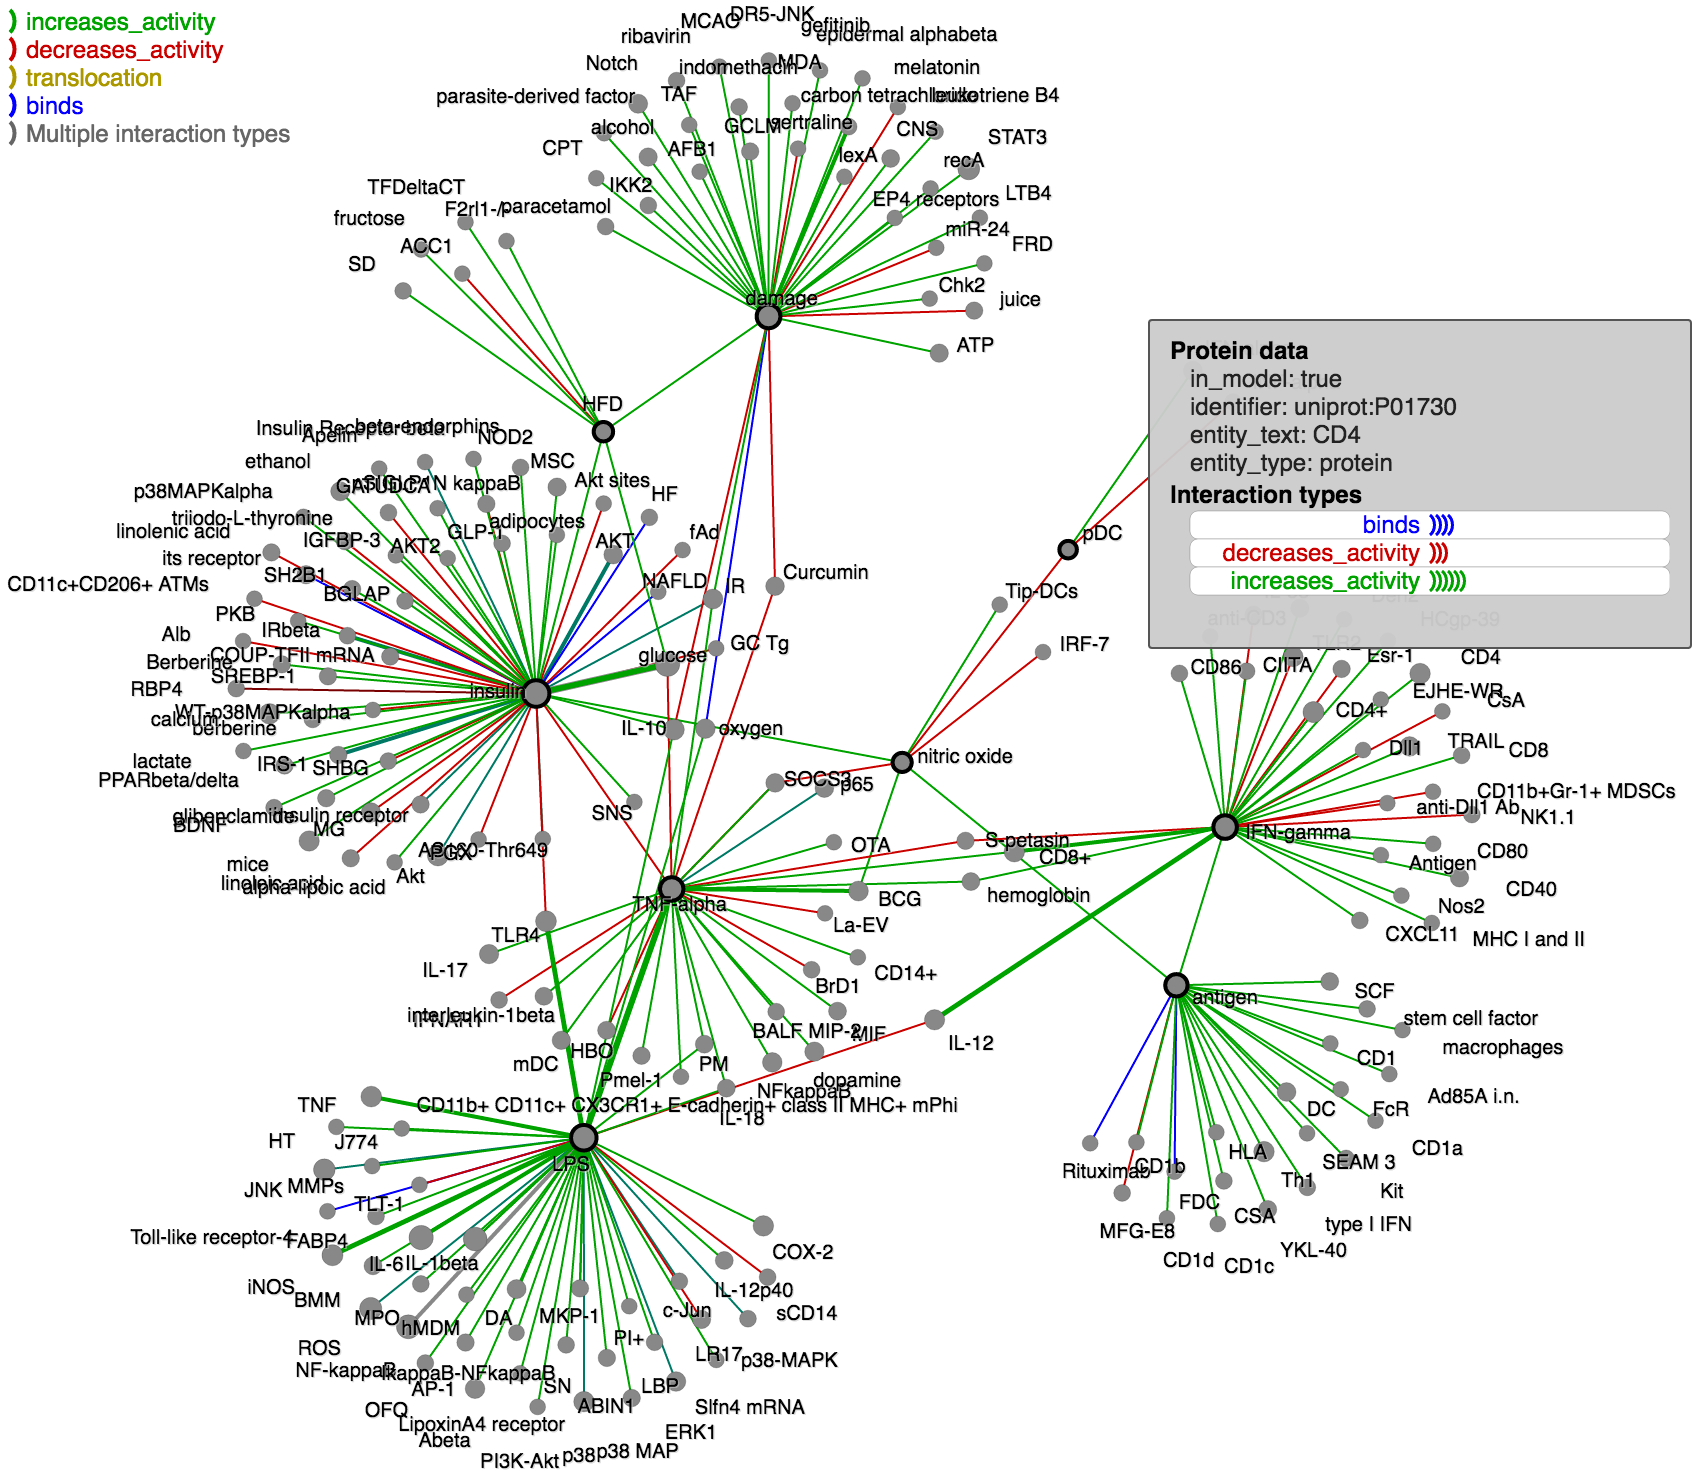
\includegraphics[width=225pt]{figures/Figure3.png}
  \caption{Main view in \theName{}: displaying protein information together with statistics of its immediate neighbors on mousing over.}
  \label{fig:Figure3}
\end{figure}

\theName{} supports finding paths between selected proteins (visualization task \textbf{T3}). Fig.~\ref{fig:Figure4} shows an example. Users specify source node (\textit{PIK3CA} protein), target node (\textit{TRAF6} protein), and the maximum number of hops in between source and target (5 hops). \theName{} displays all possible paths under that condition. The source node is pinned to the left while the target node is pinned to the right of the visualization. The shortest path from \textit{PIK3CA} to \textit{TRAF6} goes through two hops (\textit{Akt} and \textit{NF-kappaB}). By stretching source and target nodes to both sides of the force-directed layout, the shortest path is usually the horizontal path from left to right. This feature is useful in visualizing shortest path and is not available in popular visualization tools such as ChiBE 2~\cite{ChiBE2_2014}, Cytoscape~\cite{shannon2003cytoscape}, and PCViz~\cite{cerami2011pathway}. 

\begin{figure}[h!]
  \centering
  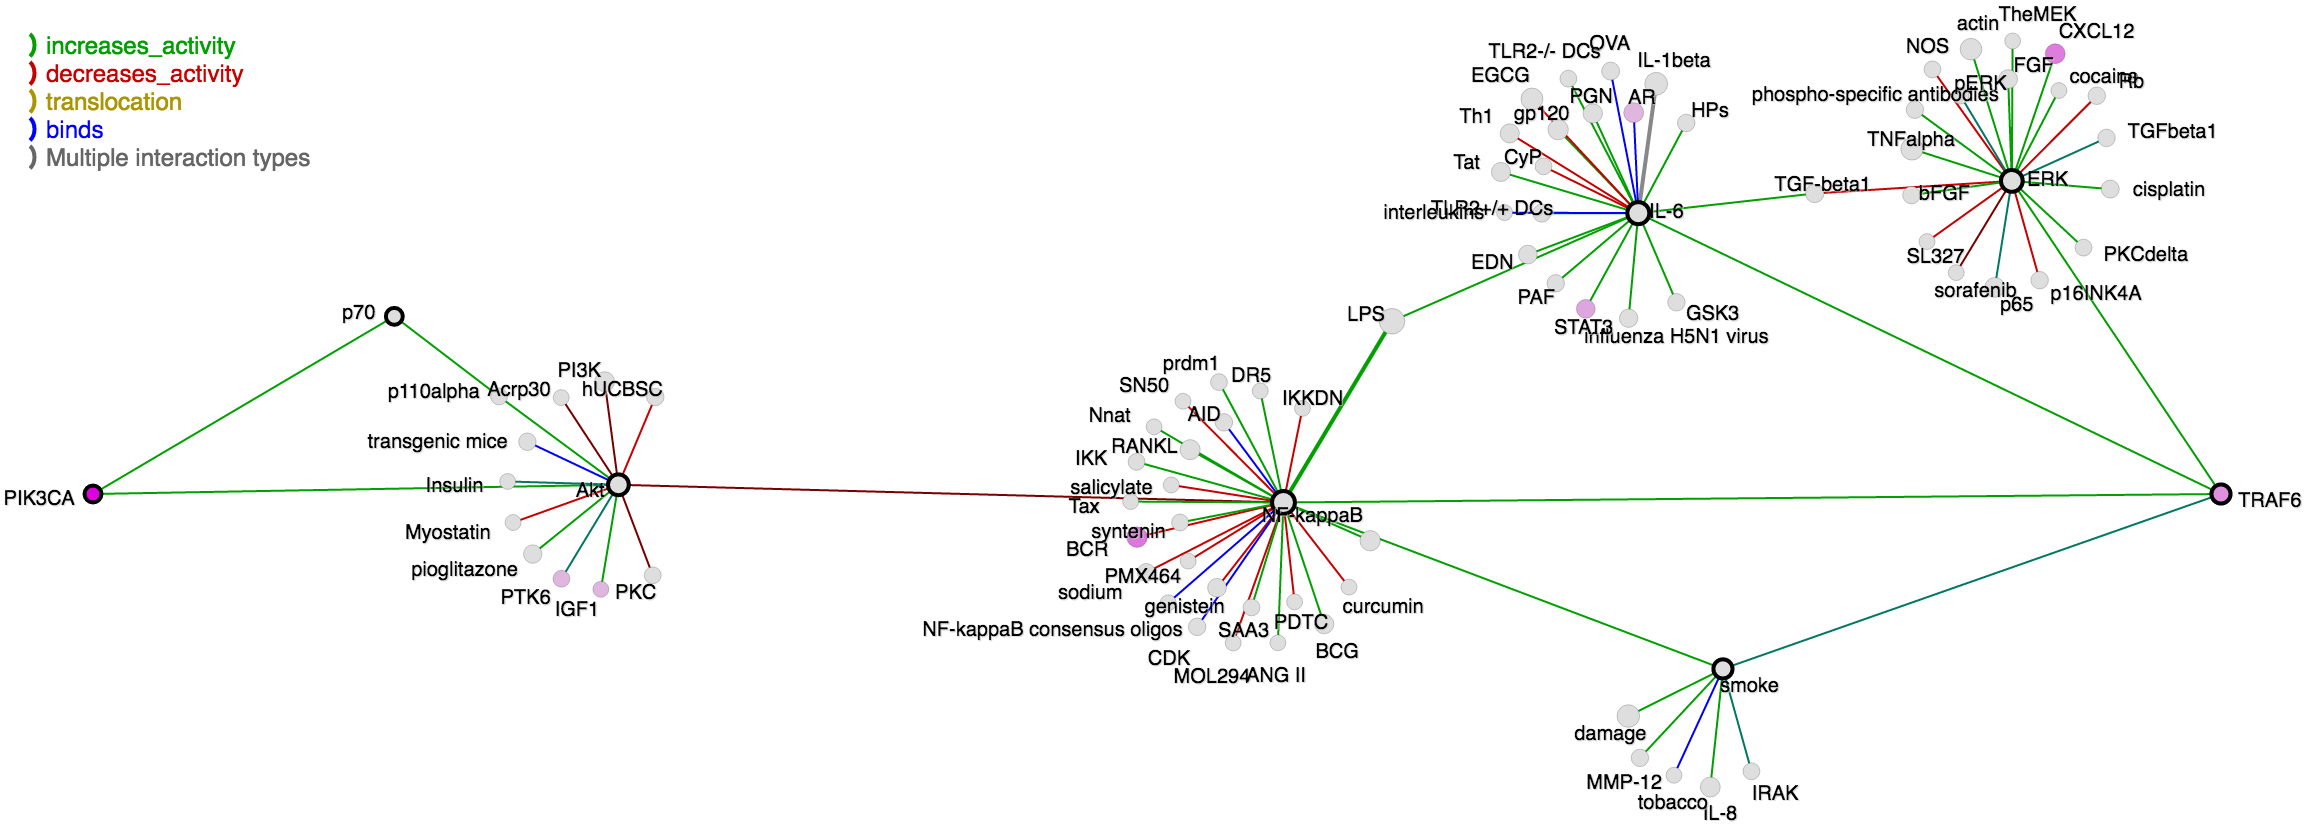
\includegraphics[width=250pt]{figures/Figure4.png}
  \caption{ Main View in \theName{}: Visualizing all possible paths from \textit{PIK3CA} (left) to \textit{TRAF6} (right) going through 5 or fewer hops.}
  \label{fig:Figure4}
\end{figure}

\theName{} also supports overlaying cancer genomics data onto the network (visualization task \textbf{T2}). In Fig.~\ref{fig:Figure4}, purple nodes are proteins with high copy number alteration in the Bladder Urothelial Carcinoma study (TCGA, Nature 2014). Notice that both source and target nodes are highly altered in this cancer study. \theName{} accesses this cancer study on cBioPortal through its web service interface (described in Section~\ref{sec:cBioPortal})

\subsection{Context View}
\label{sec:ContextView}
Working definition of context in text: An instance of context is a single assertion about species (such as human, mouse, and yeast), organ, tissue type, cell-line that holds across some region of text; any mechanism components mentioned in that region acquire that context assertion as a property. 

Systems biologists and cancer researchers are frequently interested in understanding the contexts of biochemical reactions and comparing protein interaction sub-networks by context (visualization task \textbf{T4}). The left panel in Fig.~\ref{fig:Figure5}(a) shows stacking plots~\cite{Dang2010Stacking} in our context view for the network in the main view (right panel). In particular, we show a 2-degree separation network of a selected protein (\textit{antigen}) which is located in the center of the main view. Fig.~\ref{fig:Figure5}(b) depicts brushing and linking of two views. We have selected \textit{mouse} in the \textit{species} category. Other context categories are updated accordingly. In the main view (on the right), we notice that all protein interactions in \textit{mouse} are between \textit{antigen} and its immediate neighbors, but not the second degree separated neighbors.  

\begin{figure}[h!]
  \centering
  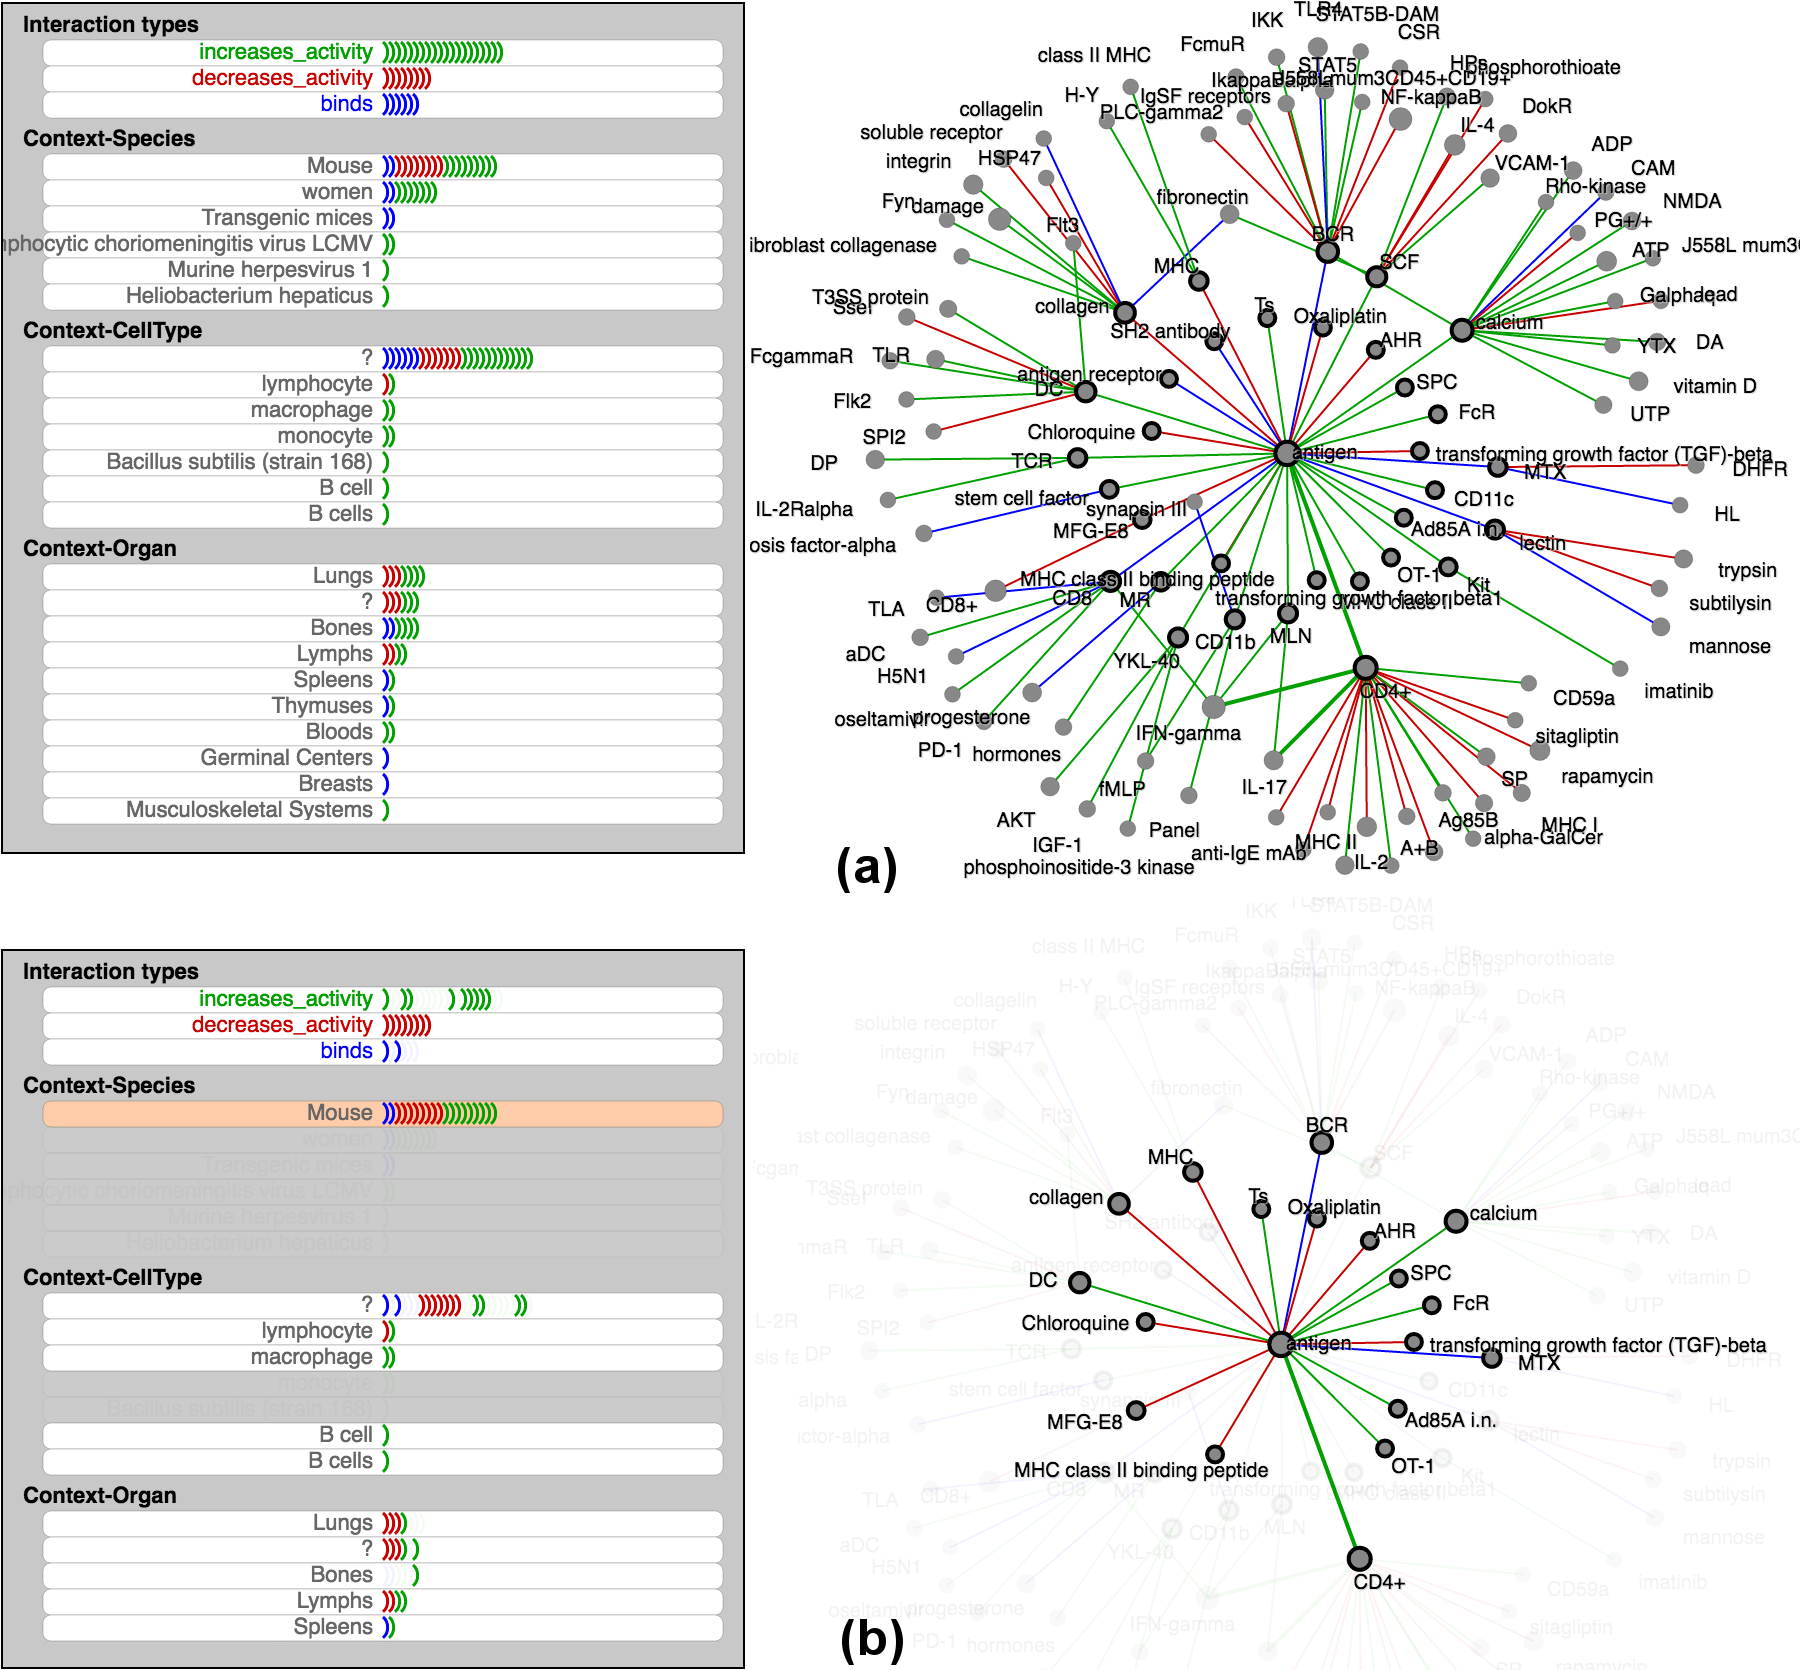
\includegraphics[width=225pt]{figures/Figure5.png}
  \caption{ Visualizing and interacting with context view in \theName{}: (a) Stacking plots (left) by species, cell type, and organ of the 2-degree separation network of \textit{antigen} (right) (b) Selecting \textit{mouse} in context view.}
  \label{fig:Figure5}
\end{figure}


\subsection{Publication View}
\label{sec:PublicationView}
We use TimeArcs visualization~\cite{Dang2016TimeArcs} to show the discoveries of these index cards by publication year. A request to load relevant publications for new index cards is sent to the PMC publication database on our server every time the protein network is expanded.
Fig.~\ref{fig:Figure6}(b) shows an example of publication view of the graph in Fig.~\ref{fig:Figure6}(a). In particular, the time axis goes from left (2004) to right (2012). An arc connects two proteins/complexes at a particular time (based on when the interaction was discovered/ publication year). The link colors encode interaction types. 

\begin{figure}[h!]
  \centering
  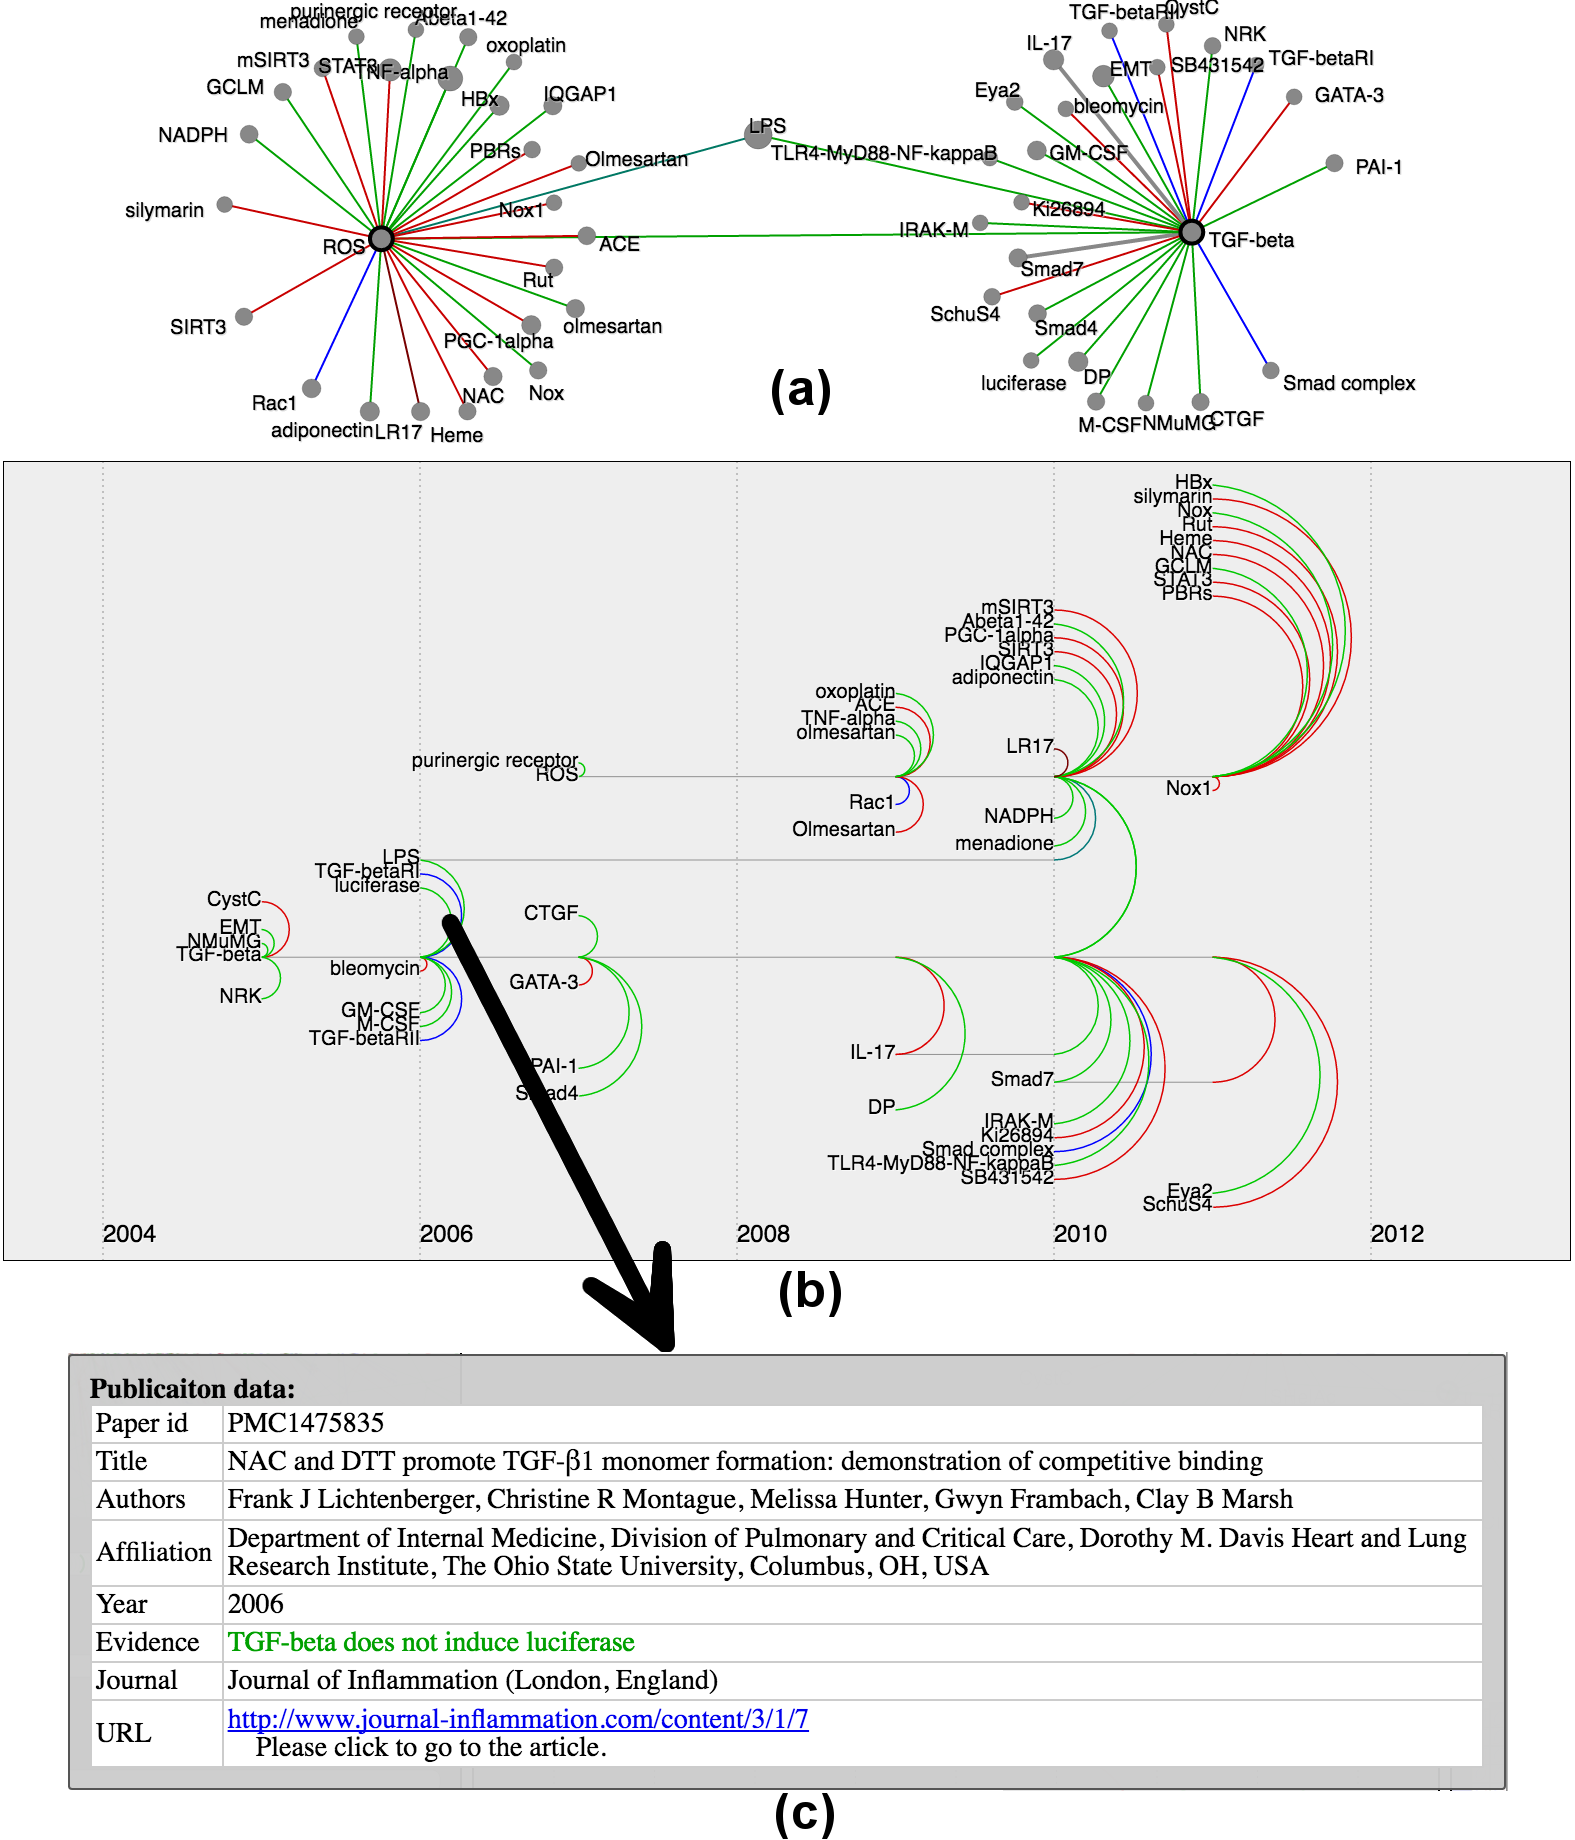
\includegraphics[width=225pt]{figures/Figure6.png}
  \caption{ Visualizing and interacting with publication view in \theName{}: (a) Sub-network of \textit{TGF-beta} and \textit{ROS} proteins in the main view (b) Publication view of the same data where time axis goes from left to right (c) Publication pop-up window when mousing over an arc in the publication view (at the origin of the arrow).
  }
  \label{fig:Figure6}
\end{figure}

Mousing over a protein name displays all publications related to that protein. As depicted in Fig.~\ref{fig:Figure6}(c), mousing over an arc displays publication data associated with an index card, such as paper title, authors' names, authors' contacts, affiliations, publication year, journal name, and external link. Users can go to the actual paper by clicking on the provided link. Notice that the evidence (the actual text in this paper where the protein interaction was extracted from) is highlighted in a different color (the color used to encode that interaction type). The user can also request to show the publication chart over time of a selected protein in our entire PMC publication database. (The earliest publications archived by PMC relevant to biological pathways date back to more than 60 years ago.)

\subsection{Conflict Matrix}
\label{sec:ConflictMatrix}
We use the index card comparator script on our server to detect potential conflicts between index cards in the main view. In Fig.~\ref{fig:Figure7}, \textit{TGF-beta} is selected and iteratively expanded. The index card comparison results are presented in the form of an adjacency matrix. Index cards in the conflict matrix are ordered by interaction type. In each cell, we draw an arc symbol for each interaction (colored by type) of the two participating index cards as depicted in the left panel of Fig.~\ref{fig:Figure7}(a). The cell backgrounds are colored by the results returned from the comparator script on our server (orange are index cards with potential conflict). In Fig.~\ref{fig:Figure7}(b), we inspect a potential conflict cell in the matrix (left). Two corresponding index cards are highlighted in the publication view (right). As depicted, the two index cards have the same participants (\textit{TGF-beta} and \textit{Smad7}), but opposite interaction types (\textit{increase\_activity} versus \textit{decrease\_activity}). This indicates conflicting knowledge obtained from two different publications in 2010 and 2011. We now look further into details of publication data for each index card to verify these conflicting information as shown in Fig.~\ref{fig:Figure7}(c). 

\begin{figure}[h!]
  \centering
  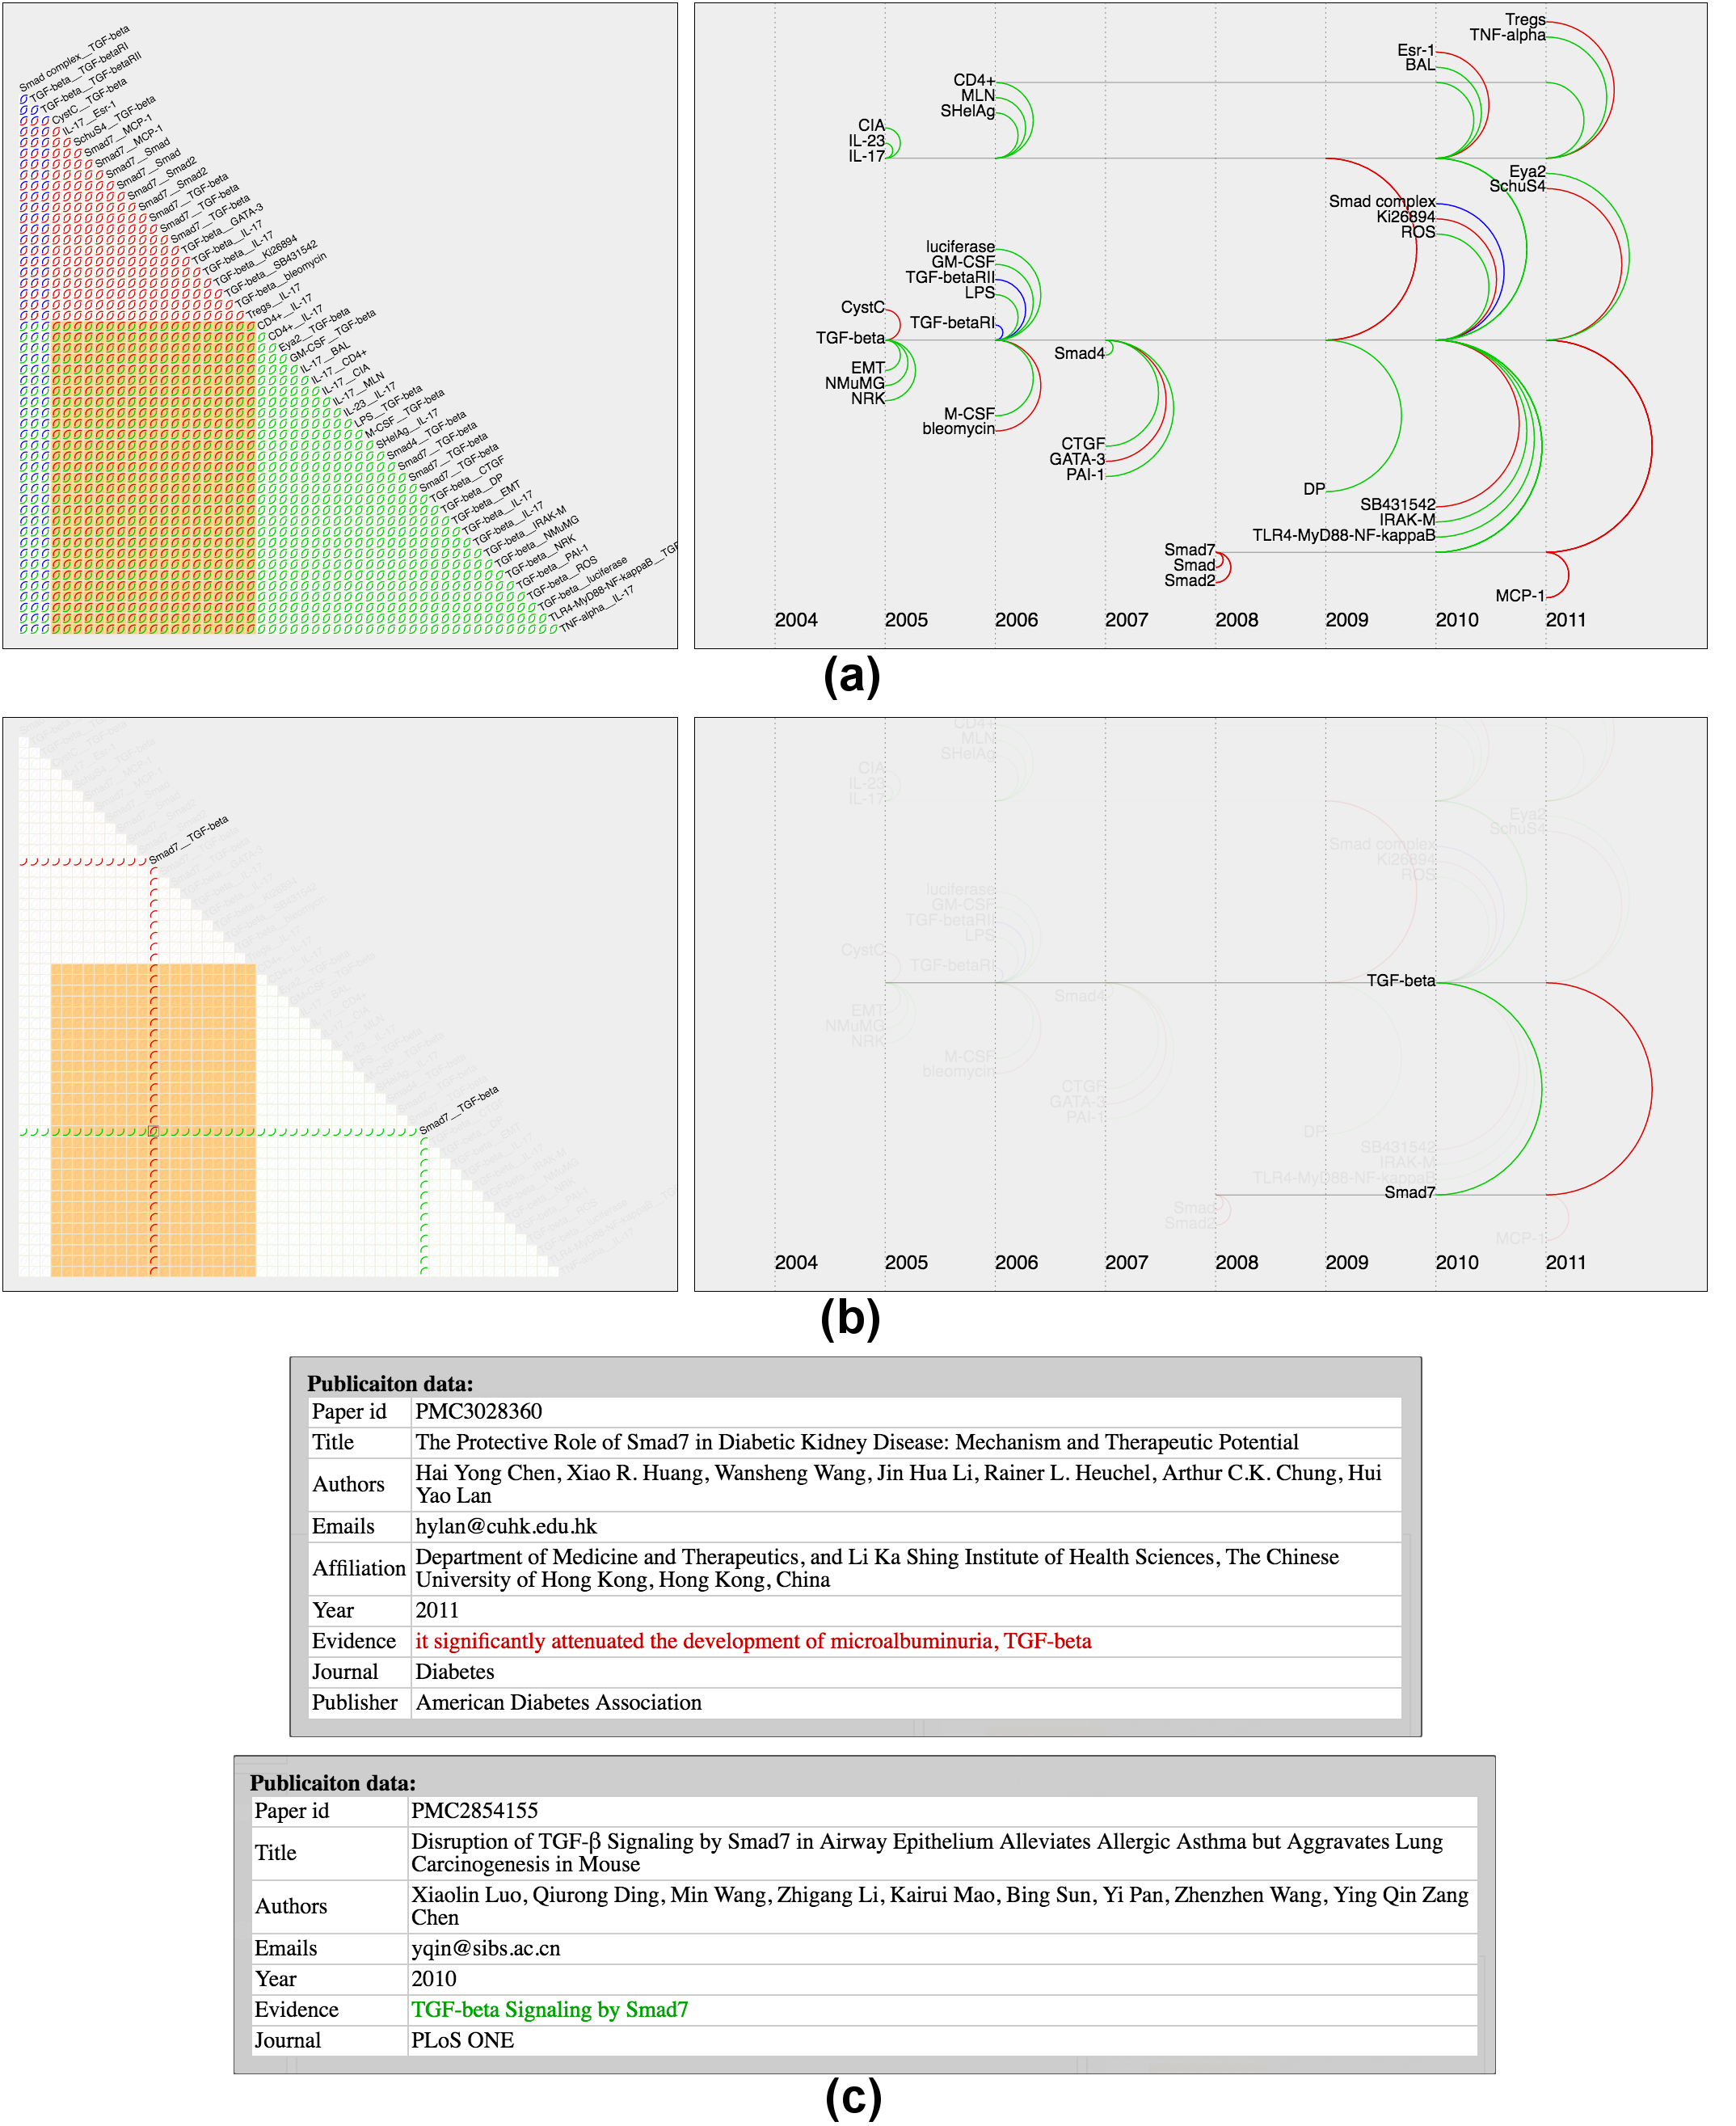
\includegraphics[width=225pt]{figures/Figure7.png}
  \caption{ Visualizing and interacting with conflict matrix in \theName{}: (a) Conflict matrix (left) and publication view (right) of the \textit{TGF-beta} sub-network (b) Linking conflict matrix (left) and publication view (right) on mousing over a potential conflict cell (between two compared index cards) in the matrix (c) Publication data of the two highlighted index cards in (b).
  }
  \label{fig:Figure7}
\end{figure}

\section{Results and Discussion}

\subsection{Comparison of \theName{} to related tools}
The matrix representation avoids edge crossings for dense networks. However, a drawback of all matrix representations is that paths between nodes are difficult to identify and trace. There are many visualization tasks related to tracing flows~\cite{biovisDang2} through protein interaction network (see visualization tasks \textbf{T1}, \textbf{T3}, and \textbf{T4}). Therefore in this section, we compare \theName{} to related node-link representations (see Table~\ref{table1}) with respect to the visualization tasks defined previously in this paper. 

\renewcommand{\arraystretch}{0.5}% Tighter
\begin{table}[htb]
     \begin{center}
     \begin{tabular}{ l c c c c c c }
     \toprule
& \textbf{T1} & \textbf{T2} & \textbf{T3} & \textbf{T4} & \textbf{T5} & \textbf{T6} \\
  \hline  
PCViz~\cite{cerami2011pathway}  &  & \cellcolor{gray!25}\checkmark & \cellcolor{gray!25}\checkmark  & & &
 \\
ChiBE 2~\cite{ChiBE2_2014} & & \cellcolor{gray!25}\checkmark  & \cellcolor{gray!25}\checkmark  &  & &
\\ 
Cytoscape~\cite{shannon2003cytoscape} &  \cellcolor{gray!25}\checkmark  &  & \cellcolor{gray!25}\checkmark &  & & 
\\ 
Extended LineSets~\cite{biovisPaduano1} & \cellcolor{gray!25}\checkmark  & & & & & 
\\ 
ReactionFlows~\cite{biovisDang2} &  
& &\cellcolor{gray!25}\checkmark  & & & 
\\ 
\theName{} &  
\cellcolor{gray!25}\checkmark& \cellcolor{gray!25}\checkmark & \cellcolor{gray!25}\checkmark & \cellcolor{gray!25}\checkmark & \cellcolor{gray!25}\checkmark & \cellcolor{gray!25}\checkmark 
\\ 
\bottomrule
\end{tabular}
      \caption{Comparisons of protein network visualization tools on six tasks.}
      \label{table1}
      \end{center}
\end{table}

This section does not mean to survey all visualization tools for biological network analysis~\cite{Suderman2007Tools,Pavlopoulos2008Survey,Huang2009Bioinformatics}. Instead, we try to cover more recent tools on the selected visualization tasks, from the common tasks in network visualization (\textbf{T1}, \textbf{T2}, and \textbf{T3}) to more recent demands from domain experts due to the emerging availability of high volume data (\textbf{T4}, \textbf{T5}, and \textbf{T6}). 


\subsection{Implementation}

\theName{} is implemented in D3.js~\cite{Bostock2011D3}. The application, source code, sample data, and demo video are provided via our GitHub project repository, located at \url{http://github.com/CreativeCodingLab/BioLinker}.


%\section{Conclusions}
%In this paper, we introduced \theName{}, a novel visualization system that helps users to perform bottom-up exploration of protein interaction networks. We also described the client-server infrastructure that handles the large amount of publication and index card data. Our database currently contains 3.5 millions index cards and 290,000 PMC publications, and these numbers will keep increasing as new information is extracted from existing articles and as new articles are archived on PMC. Since we enable a bottom-up approach, we only send requests to our server upon user request. Throughout the paper, we provided use cases where users interact with different views in \theName{}. These views are all linked to provide supplementary information.

%In the current version, \theName{} allows users to overlay cancer genomics data (such as mutation, copy number alterations, and gene expression) from a cancer study onto the network. The ability to compare and classify genes/proteins across various cancer studies using automatic feature detection~\cite{Wilkinson2005scagnostics,Dang2014Transforming} and then visualize them in \theName{} is a future research direction of this work. 


%%%%%%%%%%%%%%%%%%%%%%%%%%%%%%%%%%%%%%%%%%%%%% 
%%                                          %%
%% Backmatter begins here                   %%
%%                                          %%
%%%%%%%%%%%%%%%%%%%%%%%%%%%%%%%%%%%%%%%%%%%%%%






\bibliographystyle{abbrv}
%\bibliographystyle{abbrv-doi}
%\bibliographystyle{abbrv-doi-narrow}
%\bibliographystyle{abbrv-doi-hyperref}
%\bibliographystyle{abbrv-doi-hyperref-narrow}
%%use following if all content of bibtex file should be shown
%\nocite{*}
\bibliography{bibliography}
\end{document}

